\documentclass{report}
\usepackage{graphicx}
\usepackage{sidecap}
\usepackage{fancyhdr}
\usepackage{lscape}
\usepackage[absolute]{textpos}
\usepackage{SIunits}
\usepackage{sistyle}
\usepackage{amsmath}
\usepackage{french}

\makeatletter
\def\maketitle{%
  \null
  \thispagestyle{empty}%
  \vfill
  \begin{center}\leavevmode
    \normalfont
    {\LARGE \@title\par}%
    \vskip 1cm
    {\Large \@author\par}%
    \vskip 1cm
    {\Large \@date\par}%
  \end{center}%
  \vfill
  \null
  \newpage
  }
\makeatother
\author{Groupe : Mattens Simon, Dom Eduardo \\ BAB2 Sciences Informatiques}
\title{Rapport : Mesures au moyen d'un oscilloscope}
\date{\today}


\begin{document}
\maketitle

\section*{1 Introduction}
\hspace*{0.5cm}
Le but de la manipulation est 
d'une part, mesurer des hauteurs et des dur\'ees de signaux, des d\'ephasages entre deux signaux de m\^eme fr\'equence, observer des figures de Lissajous et faire la distinction entre tension efficace et tension maximale et d'autre part, r\'ealiser des circuits \'electronique \`a base de diodes, de capacit\'e et de r\'esistance en vue de mesurer diff\'erentes tension. C'est aussi se familiariser avec divers instruments couramment utilis\'e en \'electronique tels que l'oscilloscope et le g\'en\'erateur.

\section*{2 R\'esum\'e th\'eorique}
\subsection*{2.1 L'oscilloscope}
\hspace*{0.5cm}
L'oscilloscope permet de visualiser 2 signaux de tensions \'electriques U1 et U2 en fonction du temps. Il se branche en parall\`ele dans un circuit. Il y a aussi le mode Lissajous qui permet la repr\'esentation graphique du signal U1 en fonction du signal U2.
\subsection*{2.2 Diode}
\hspace*{0.5cm}
Composant \'electrique constitu\'e d'une jonction p-n qui ne laisse passer le courant que dans un seul sens. L'application d'une tension continue ,dont le p\^ole positif est reli\'e \`a la r\'egion p du semi-conducteur (polarisation directe), abaisse la barri\`ere de potentiel et permet le passage du courant.
\subsection*{2.3 Formules}
\hspace*{0.5cm}
Pour calculer la fr\'equence d'un signal, nous pouvons utiliser cette formule:

\begin{equation}
   frequence = \frac{1}{periode}
\end{equation}

La tension efficace peut \^etre obtenue via cette formule ci-dessous:

\begin{equation}
   Ueff = \frac{Umax}{\sqrt{2}}
\end{equation}

La vitesse angulaire est donn\'ee par :

\begin{equation}
    \omega = 2\cdot \pi \cdot f   
\end{equation}

La tangente du d\'epahasage d'un signal:

\begin{equation}
    \tan(\phi) = \frac{1}{\omega RC}
\end{equation}

\section*{3 Dispositif exp\'erimental}
\hspace*{0.5cm}
Pour ce laboratoire, nous avons eu \`a notre disposition deux g\'en\'erateurs, un oscilloscope, deux c\^ables pour connecter les deux g\'en\'erateurs \`a l'oscilloscope, une pince croco pour mesurer les tensions \`a des endroits pr\'ecis du circuit, un multim\`etre, une fiche banane, une r\'esistance, un condensateur, une plaque \'electronique et deux circuits d\'ej\`a faits repr\'esentant le pont de Gratz pour l'un et un redresseur simple pour l'autre.
\\
\\
Nous avons utilis\'e diff\'erentes fr\'equences et \'echelles pour nos observations.
\begin{itemize}

\item Pour la partie E1.3.1, nous avons utilis\'e une frequence de 500Hz fix\'e sur le g\'en\'erateur. De plus, la tension maximum a \'et\'e fix\'ee entre 1 et 4 Volts. L'\'echelle de temps (l'axe X) , fix\'ee sur l'oscilloscope pour visualiser correctement les signaux, est de 1ms.
\item Conform\'ement \`a l'\'enonc\'e, la frequence du g\'en\'erateur a \'et\'e fix\'ee \`a 50Hz et la tension maximale de l'oscilloscope \`a 5 Volts pour la seconde partie du laboratoire (E1.3.2). L'\'echelle de temps utilis\'ee est de 2ms.
\item Pour le reste du laboratoire, nous avons utilis\'e une fr\'equence de 1000Hz et une \'echelle de temps de 2ms. Lorsque les manipulations demandaient deux g\'en\'erateurs, l'un \'etait fix\'e \`a 1000 Hz et l'autre variait entre 1000 et 5000Hz.
\end{itemize} 



\section*{4 Prise des mesures \& r\'esultats}
\subsection*{4.1) E1.3.1: Visualisation de tensions alternatives}
\hspace*{0.5cm}
Apr\`es avoir fix\'e la fr\'equence du g\'en\'erateur \`a 500 Hz et Umax entre 1 et 4 Volts, on a visualis\'e les trois formes de signaux: sinusoidale, triangulaire et carr\'ee. Nos difficullt\'es ont \'et\'e de trouver les bons boutons, de "stopper" les graphes affich\'es sur l'oscilloscope ainsi que de calculer la p\'eriode. En effet il a \'et\'e difficile de se familiariser aux graduations de l'oscilloscope.
\\
On a mesur\'e une p\'eriode de 0,002 secondes. De cette observation, on peut ais\'ement calculer la fr\'equence en utilisant la formule suivante:
\begin{equation}
   frequence = \frac{1}{periode}
\end{equation}
On obtient:

\begin{equation}
   frequence = \frac{1}{0,002}
\end{equation}

\begin{equation}
   \Leftrightarrow frequence = 500 \hertz
\end{equation}

\`A l'aide du multim\`etre utilis\'e en voltm\`etre, nous avons mesur\'e, au moyen d'un c\^able \`a fiche banane, la tension efficace du g\'en\'erateur Ueff (tension alternative sinusoidale).
\begin{equation}
   Ueff = 1.449 V
\end{equation}

Sachant que Umax = 2V, nous avons su \'etablir la relation liant Umax et Ueff dans le cas d'une tension alternative sinusoidale.

\begin{equation}
   Ueff = \frac{Umax}{\sqrt{2}}
\end{equation}

Nous pouvons v\'erifier notre relation en utilisant les valeurs mesur\'ees:

\begin{equation}
   Ueff = 1,449 = \frac{Umax}{\sqrt{2}}
\end{equation}

\begin{equation}
   Umax = 1,449 \cdot \sqrt{2} = 2,049 V
\end{equation}
Notons que Umax n'est pas \'egale \`a 2 d\^u \`a l'erreur de mesure.
\\

Nous avons mesur\'e la tension efficace du signal triangulaire qui est de 1.235 Volts et la tension efficace du signal carr\'e de 2.27 Volts.

\subsection*{4.2) E1.3.2: \'Etude d'un circuit redresseur simple (1 diode)}
\hspace*{0.5cm}
\begin{figure}[ht!]
\centering
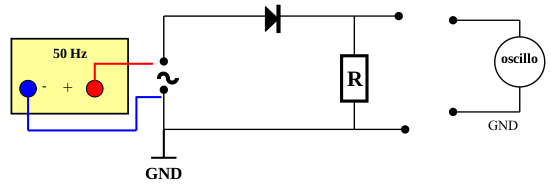
\includegraphics[width=90mm]{circuitE1.3.2.jpg}
\caption{Circuit redresseur simple}
\label{overflow}
\end{figure}
\\
Apr\`es avoir identifi\'e tous les \'el\'ements du circuit mis \`a notre disposition(voir ci-dessus), nous avons mesur\'e la tension aux bornes du circuit \`a l'aide d'un c\^able croco.

\begin{equation}
   tension = \text{ hauteur du signal}[m] \cdot \text{ unit\'e}[V]
\end{equation}
Nous avons choisi 5 Volts comme unit\'e( r\'egl\'e sur l'oscilloscope). La hauteur du signal est en fonction de l'unit\'e choisie.

\begin{equation}
   \Leftrightarrow tension = 2,4 \cdot 5 = 12 V
\end{equation}

Nous constatons que le calcul de la tension aux bornes de la r\'esistance Ur est identique au calcul de la tension appliqu\'ee aux bornes du circuit. La tension aux bornes de la r\'esistance est donc de 12V.

\subsection*{4.3) E1.3.3: \'Etude d'un circuit redresseur en pont (pont de Gratz)}
\hspace*{0.5cm}
\begin{figure}[ht!]
\centering
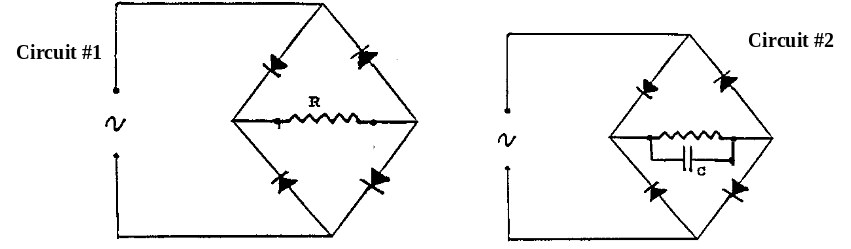
\includegraphics[width=90mm]{circuitE1.3.3.jpg}
\caption{circuit redresseur de pont sans capacit\'e (circuit 1) et avec capacit\'e (circuit 2)}
\label{overflow}
\end{figure}
\\

Nous avons utilis\'e le circuit redresseur en pont pour visualiser le signal au bornes de R gr\^ace \`a l'oscilloscope. Ensuite, nous avons plac\'e , en s\'erie, une capacit\'e de 5 \micro F pour observer l'effet sur la forme du courant obtenu. On pr\'evoit que le courant, aux abords de la r\'esistance, va diminuer sensiblement.
Le but final est d'avoir du courant continu.

\subsection*{4.4) E1.3.4: Visualisation de 2 signaux sinuso\¨idaux de m\^eme fr\'equence d\'ephas\'es}
\hspace*{0.5cm}
\begin{figure}[ht!]
\centering
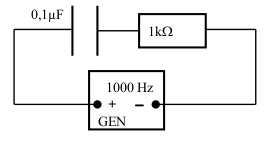
\includegraphics[width=90mm]{circuitE1.3.4.jpg}
\caption{Circuit RC}
\label{overflow}
\end{figure}
\\

Nous avons r\'ealis\'e le circuit RC tel que sp\'ecifi\'e dans l'\'enonc\'e. On a donc plac\'e en s\'erie une r\'esistance de $1 k\ohm$  et un condensateur de 0,1\micro\farad. Nous avons ensuite plac\'e une pince croco aux bornes de la capacit\'e et une pince croco aux bornes de la r\'esistance. Nous avons ensuite visualis\'e simultan\'ement la tension appliqu\'ee au circuit ainsi que la tension aux bornes de la r\'esistance sur l'oscilloscope.

Calculons maintenant le d\'ephasage entre ces deux signaux:
Nous constatons que l'oscilloscope a 5 divisions.
Or nous visualisons qu'un des signaux est d\'ephas\'e  de 4/5 de division. On obtient donc:

\begin{equation}
    dephasage = \frac{4}{5} \cdot \frac{1}{5}
\end{equation}

\begin{equation}
    \Leftrightarrow dephasage = \frac{4}{25} \text{ de p\'eriode}
\end{equation}

\begin{equation}
    \Leftrightarrow dephasage = \frac{4}{25} \cdot 360 = 57,6 \text{ degr\'es}
\end{equation}

Que vaut la valeur th\'eorique ?

\begin{equation}
    \tan(\phi) = \frac{1}{\omega RC}
\end{equation}

Par le rappel th\'eorique, on sait que  est la vitesse angulaire vaut:

\begin{equation}
    \omega = 2\cdot \pi \cdot f   
\end{equation}

Sachant que la fr\'equence utilis\'ee par le g\'enerateur est de 1000 \hertz, nous avons:

\begin{equation}
    \Leftrightarrow \omega = 2 \cdot \pi \cdot 1000 = 6283,185 \frac{rad}{s}
\end{equation}

On sait par l'\'enonc\'e que:
\begin{equation}
    R = 1\kilo\ohm \text{ et } C = 0,1\micro\farad 
\end{equation}

On peut r\'e\'ecrire l'\'equation (13):

\begin{equation}
    \tan(\phi) = \frac{1}{6283,185 \cdot 1000 \cdot 0,0000001}
\end{equation}

\begin{equation}
    \Leftrightarrow \tan(\phi) = 1,5915 rad
\end{equation}

\begin{equation}
    \Leftrightarrow \phi = \arctan (1,5915)
\end{equation}

\begin{equation}
    \Leftrightarrow \phi = 57,8572 \text{ degr\'es}
\end{equation}

\subsection*{4.5) E1.3.5: Observation d'un signal en fonction de l'autre: mesure pr\'ecise du d\'ephasage}
\hspace*{0.5cm}
Apr\`es avoir lu attentivement la m\'ethode de calcul pour calculer le d\'ephasage de mani\`ere pr\'ecise, nous avons observ\'e sur l'\'ecran de l'oscilloscope une ellipse dans le quadrants 1 et 3.
\hspace*{0.5cm}
\begin{figure}[ht!]
\centering
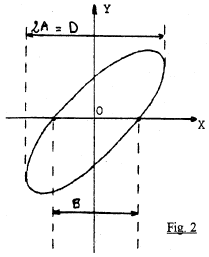
\includegraphics[width=90mm]{circuitE1.3.5.jpg}
\caption{Ellipse observ\'ee}
\label{overflow}
\end{figure}
\\

Pour une telle ellipse, le calcul du d\'ephasage est le suivant:

\begin{equation}
     \phi = \arcsin(\frac{B}{D})
\end{equation}
o\`u B est la distance entre les deux points de l'ellipse intersectant l'axe X et D 2 fois la distance entre les deux extr\'emit\'es de l'ellipse.
\\
Voici nos observations:

\begin{equation}
    D = 4,2 \text{ unit\'es et } B = 3,4 \text{ unit\'es}     
\end{equation}

On peut donc maintenant r\'e\'ecrire l'\'equation (21) avec les valeurs observ\'ees:

\begin{equation}
    \phi = \arcsin(\frac{3,4}{4,2})    
\end{equation}

\begin{equation}
    \phi = 54,04 \text{ degr\'es}   
\end{equation}

\subsection*{4.6) E1.3.6: Visualisation de signaux de fr\'equence multiple}
\hspace*{0.5cm}
La principale difficult\'e a \'et\'e de pouvoir stabiliser les figures de Lissajous. En effet, pour obtenir ces figures, nous devons changer la fr\'equence sur les deux g\'en\'erateurs \`a l'aide d'un bouton. Ce dernier est tr\`es sensible. On obtient une figure de Lissajous quand une fr\'equence d'un g\'en\'erateur est multiple de la fr\'equence de l'autre g\'en\'erateur. Ainsi, nous avons pu observer, en autre, le symbole infini apr\'es avoir fix\'e une frequence le double de l'autre.
\hspace*{0.5cm}
\begin{figure}[ht!]
\centering
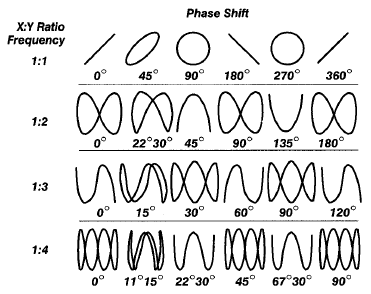
\includegraphics[width=90mm]{circuitE1.3.6.jpg}
\caption{Figures de Lissajous observ\'es}
\label{overflow}
\end{figure}
\\

\section*{5 Analyse des r\'esultats}
\subsection*{5.1) E1.3.1: Visualisation de tensions alternatives}
\hspace*{0.5cm}
On remarque que la tension calcul\'ee Umax n'est pas exactement \'egale \`a 2 Volts. En effet, la tension calcul\'ee est de 2,049V.
Calculons l'erreur de mesure :
\begin{equation}
    \epsilon = \frac{1}{5} \cdot 1ms = \frac{1}{5}Volt
\end{equation}
Or 1/5 de 2 est \'egale \`a 0,4. De ce fait, notre solution doit appartenir à l'ensemble [1,6;2,4] ce qui est bien le cas.

\subsection*{5.2) E1.3.2: \'Etude d'un circuit redresseur simple (1 diode)}
\hspace*{0.5cm}
\begin{figure}[ht!]
\centering
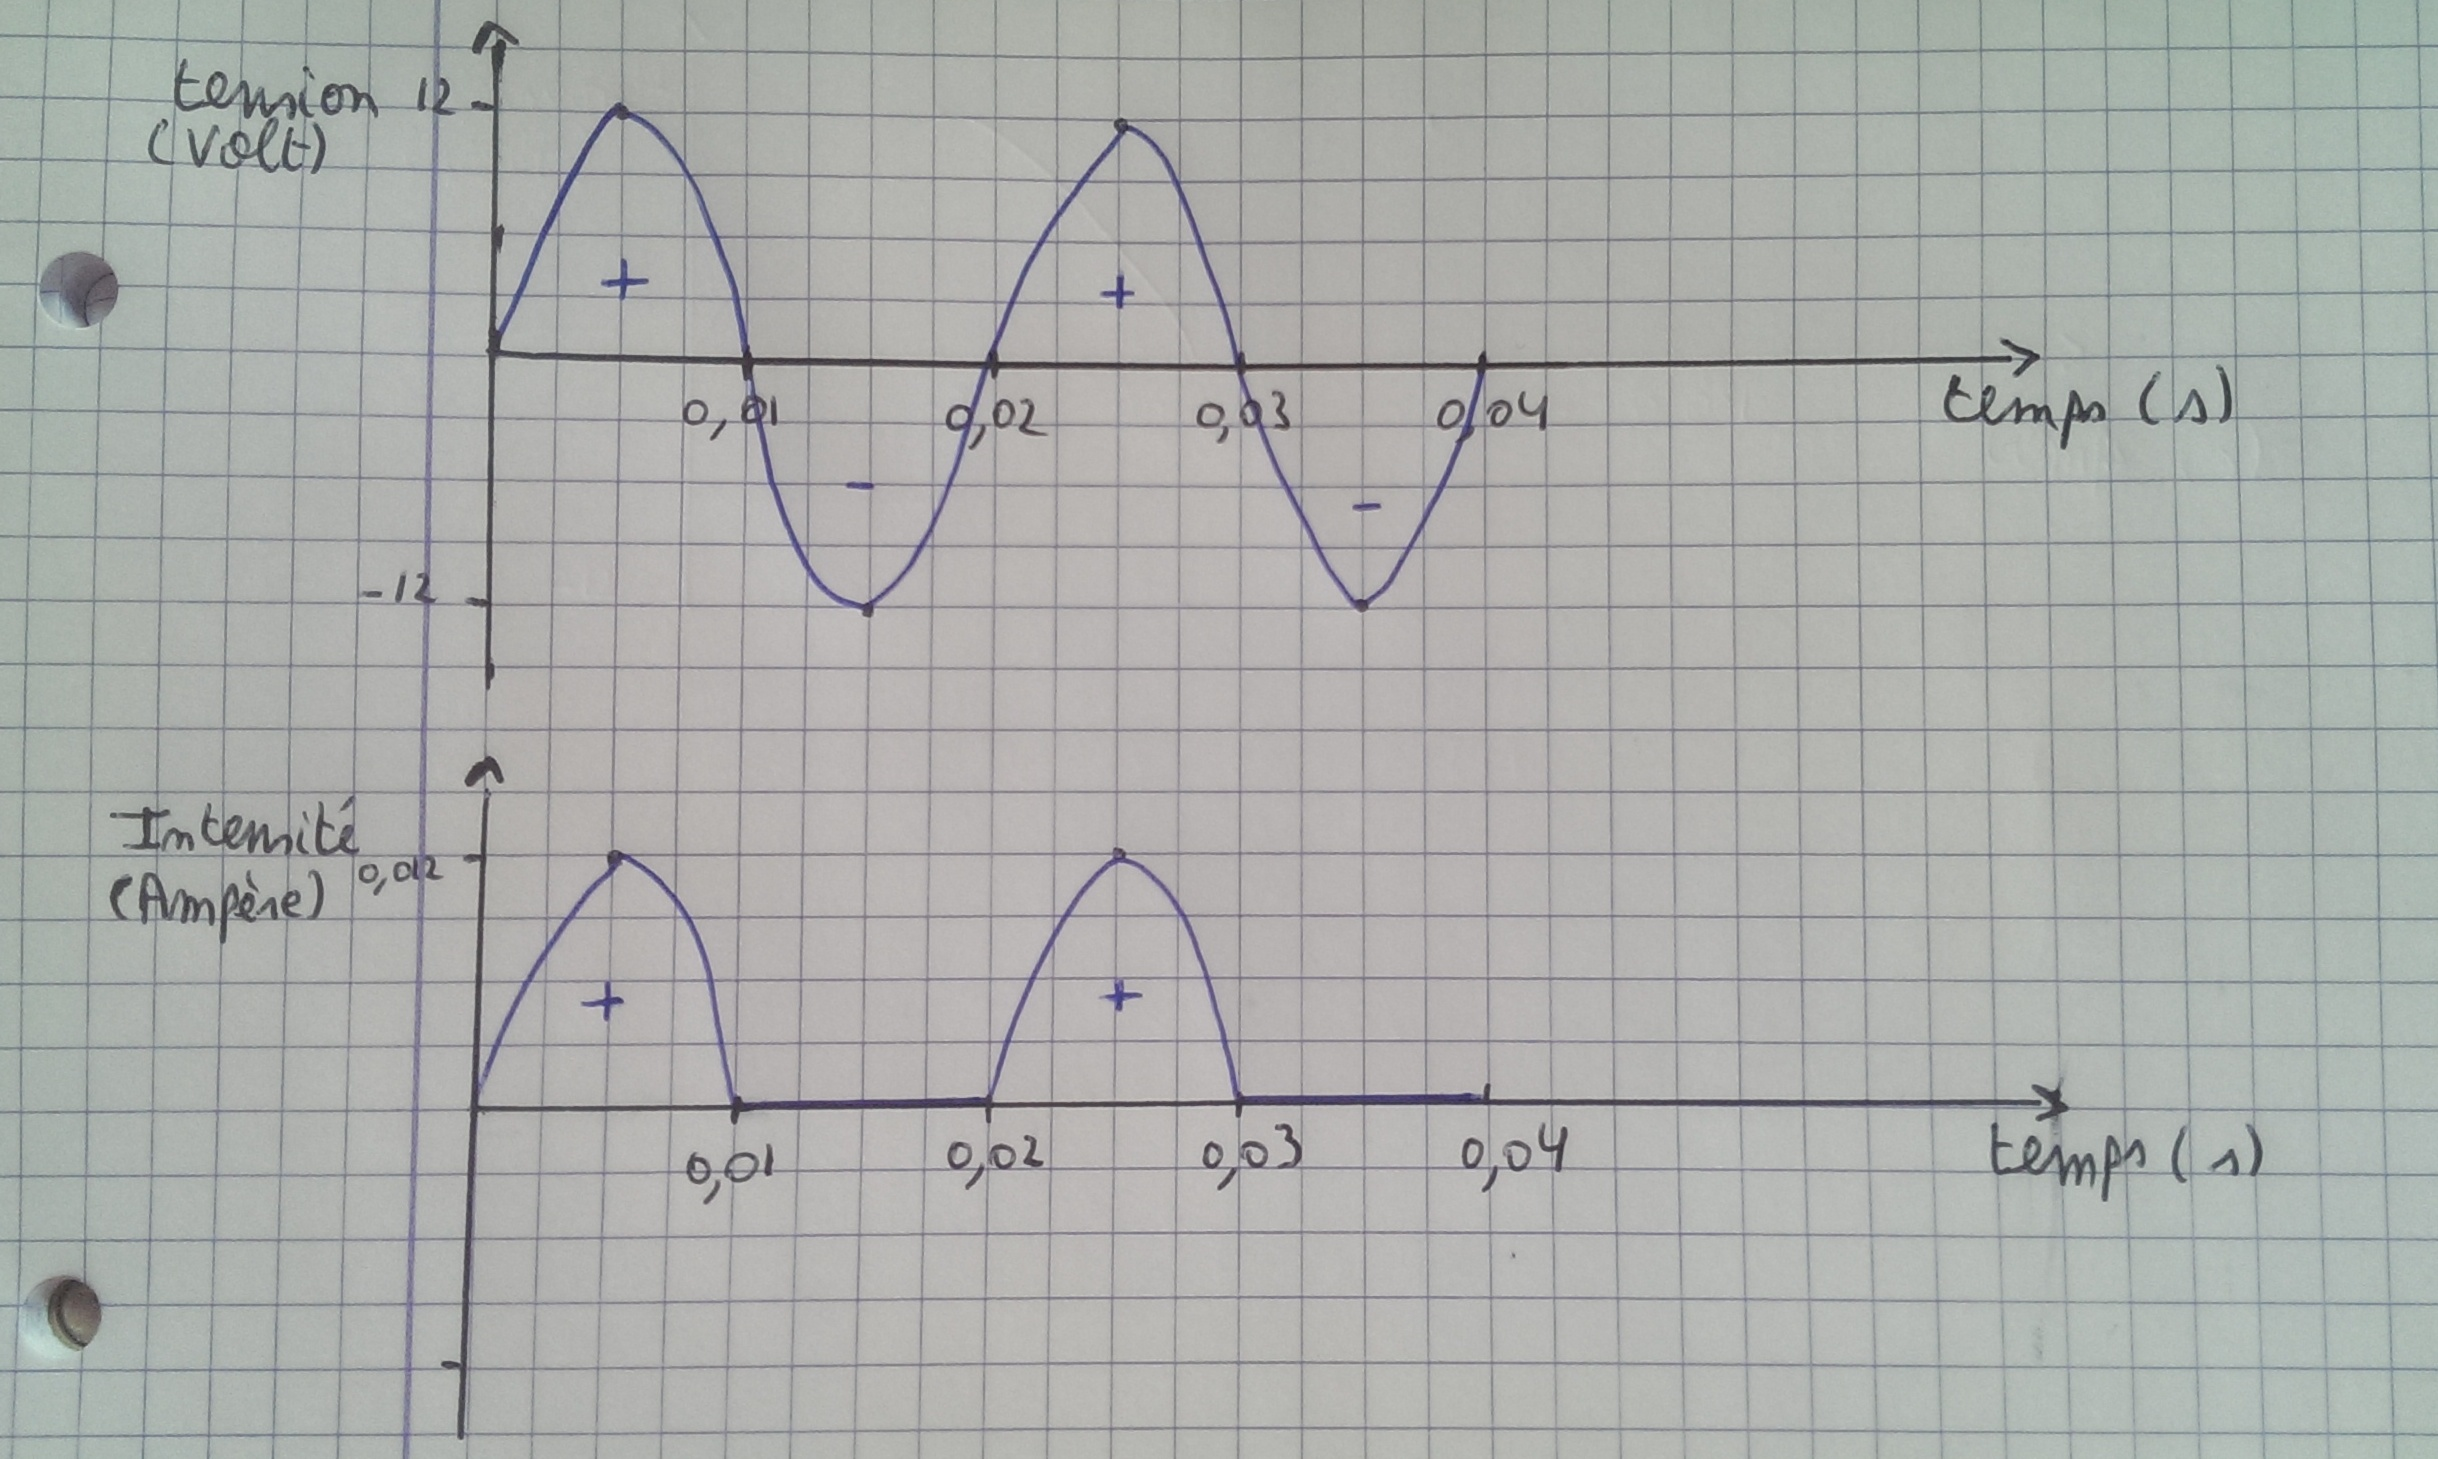
\includegraphics[width=90mm]{graphiqueE1.3.2.jpg}
\caption{Graphique du temps en fonction de la tension et graphique du temps en fonction de l'intensit\'e du courant}
\label{overflow}
\end{figure}
\\

Nous constatons que la tension oscille entre -12 et 12 Volts. La p\'eriode est de 0,02 seconde. Lorsque la tension est positive, l'intensit\'e l'est aussi. Par contre, lorsque la tension est n\'egative, l'intensit\'e du courant reste constante et est \'egale \`a 0.

Pourquoi ce ph\'enom\`ene se produit?
\\

Il y a sur le circuit redresseur simple une diode mont\'ee en s\'erie. Une diode est un composant \'electronique, constitu\'e d'une jonction p-n, qui ne laisse passer le courant que dans un seul sens, sens d\'esign\'e par la fl\`eche. On peut voir sur la figure 1 que la fl\`eche de la diode est orient\'ee de la borne + vers la borne - du g\'en\'erateur. De ce fait, la diode ne laissera passer que le courant positif et non le courant n\'egatif. C'est pourquoi, sur le graphique, lorsque la tension est n\'egative, l'intensit\'e du courant est nulle.

\subsection*{5.3) E1.3.3: \'Etude d'un circuit redresseur en pont}
\hspace*{0.5cm}
\begin{figure}[ht!]
\centering
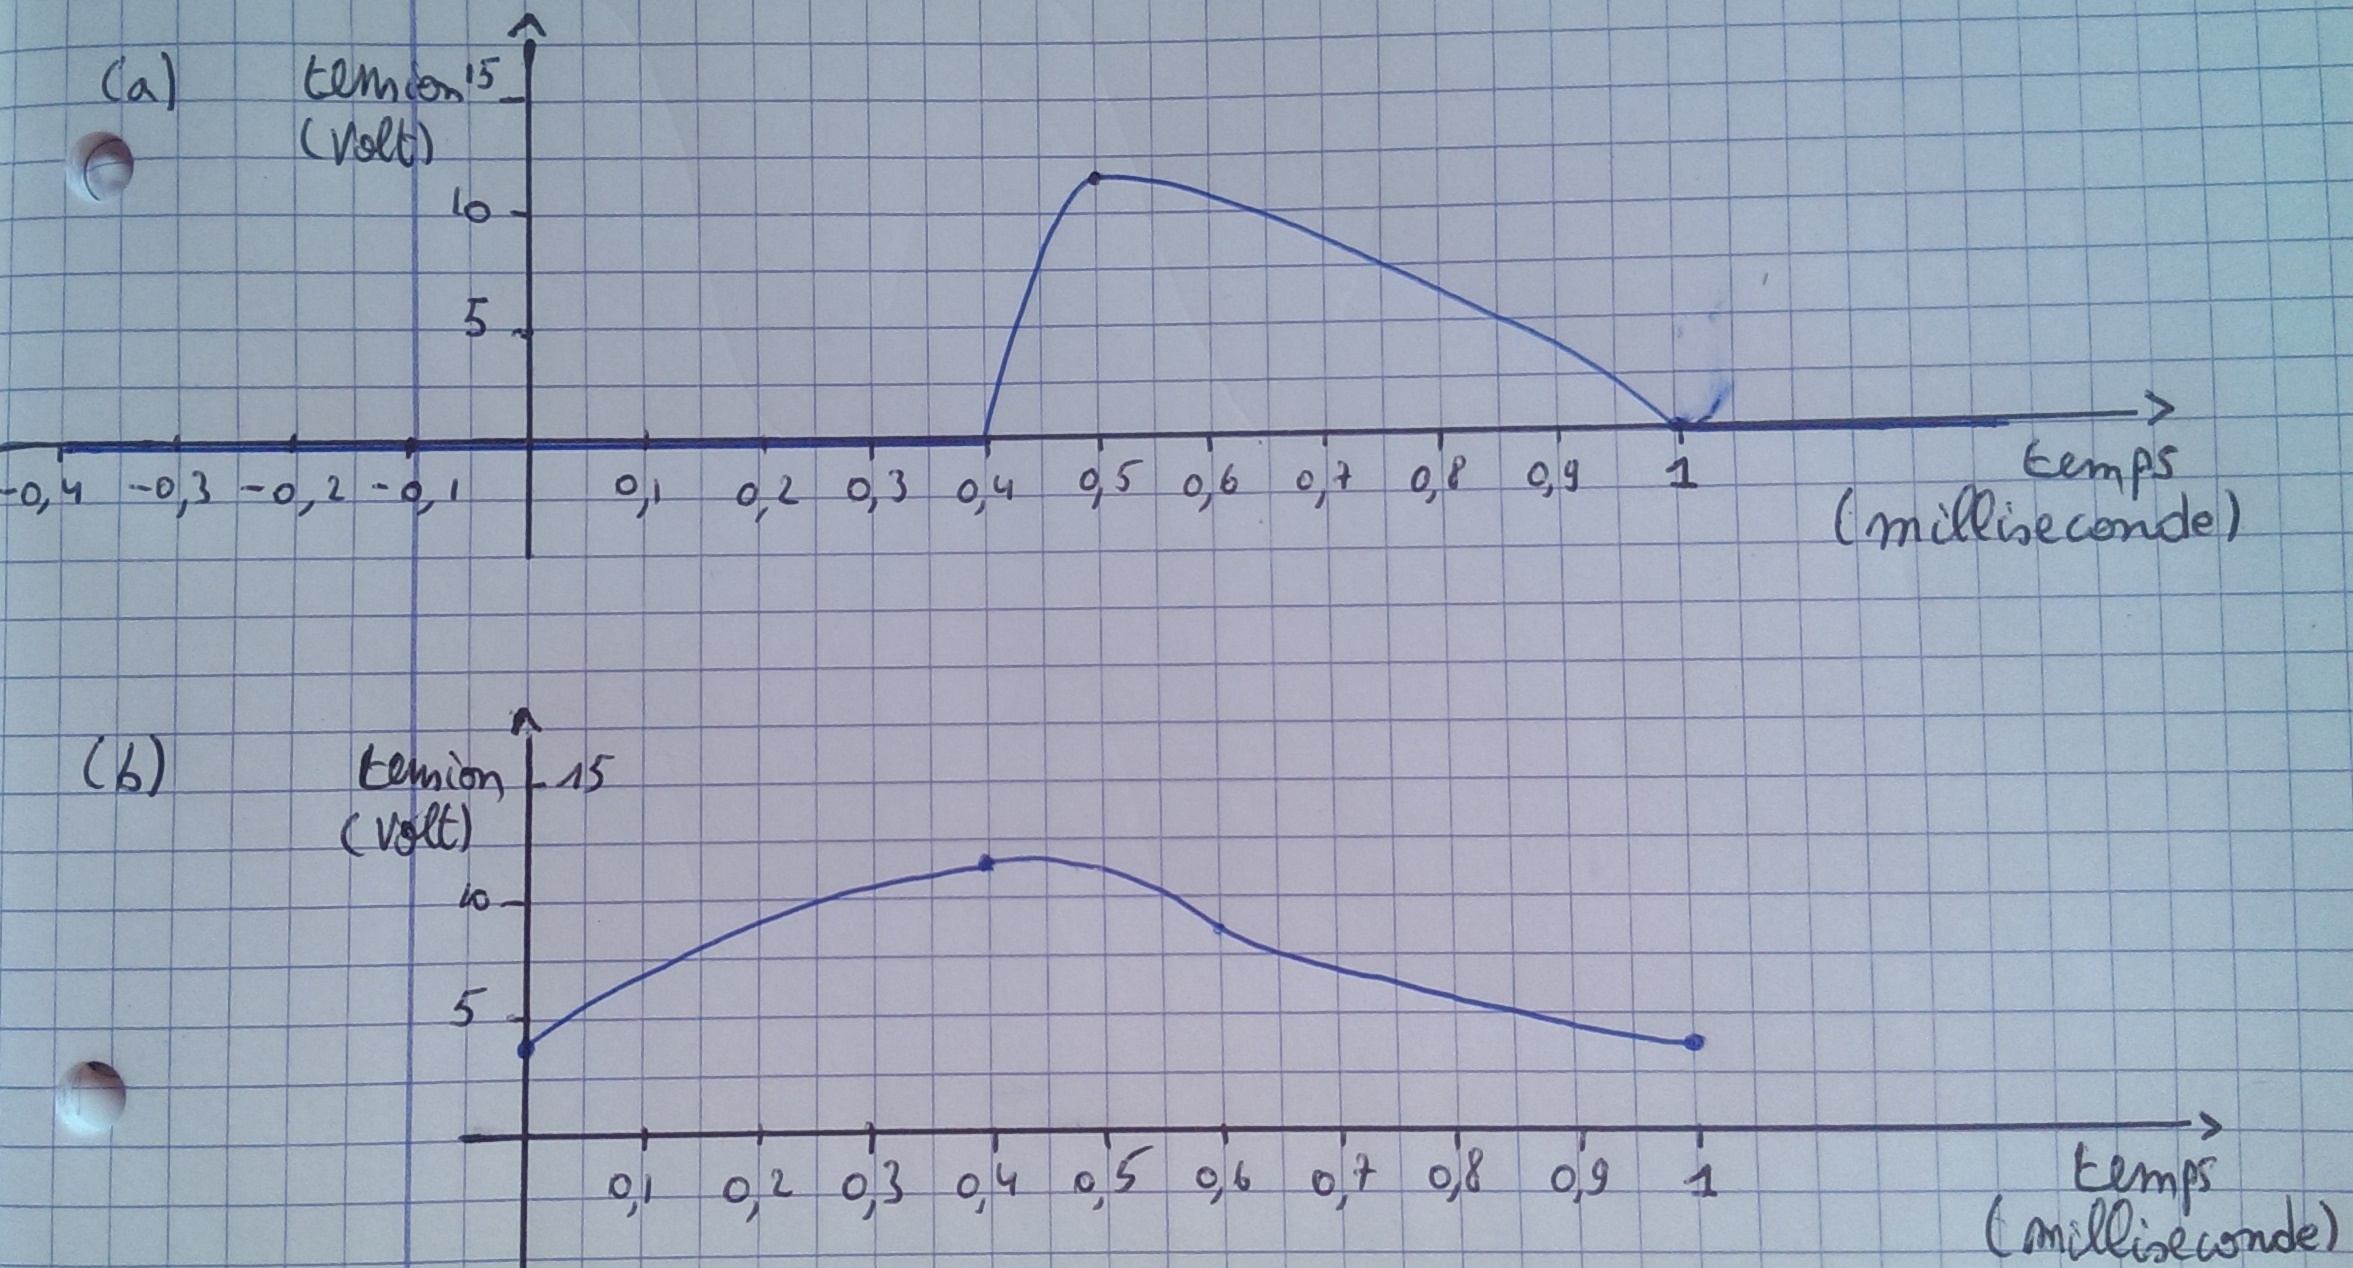
\includegraphics[width=90mm]{graphiqueE1.3.3.jpg}
\caption{Graphique(a) du temps en fonction de la tension sans capacit\'e et graphique(b) du temps en fonction de la tension avec une capacit\'e.}
\label{overflow}
\end{figure}
\\

Nos pr\'evisions \'etaient bonnes. Le courant diminue bien lorsqu'il passe dans la r\'esistance (\`a partir de 0,5ms). Avec la pr\'esence d'un condensateur dans le circuit, la diminution est moins importante et surtout, la tension ne revient pas \`a 0.
Le but final est d'avoir du courant continu.

\subsection*{5.4) E1.3.4 - E1.3.5: \'Etude d'un circuit redresseur en pont - Observation d'un signal en fonction de l'autre: mesure pr\'ecise du d\'ephasage}
\hspace*{0.5cm}
Nous obtenons un d\'ephasage de 57,6 degr\'es par observation. La valeur th\'eorique est de 57,8 degr\'es.
\\
Calculons l'erreur de mesure:
\begin{equation}
    \epsilon = \frac{1}{5}\cdot 2ms = \frac{2}{5} \text{ degr\'es}
\end{equation}
Or 2/5 de 57,8 est \'egale \`a 23,12 degr\'es. Notre valeur obtenue par observation est bien dans l'intervale acceptable. La mesure pr\'ecise du d\'ephasage est de 54,05 degr\'es. On peut donc avoir un \'ecart de 2/5 de 54,05(=21,62 degr\'es) par rapport 54,04. Notre observation est toujours correct vu l'erreur de mesure.

\subsection*{5.5) E1.3.6 Visualisation de signaux de fr\'equence multiple}
\hspace*{0.5cm}
En observant les figures de Lissajous, nous pouvons d\'eterminer le d\'ephasage d'un signal par rapport \`a l'autre en utilisant la Figure 5 du rapport. Cela permet de comparer 2 fr\'equences. En effet, par ce proc\'ed\'e, nous pouvons d\'eterminer la fr\'equence d'un signal inconnu en le comparant à un signal de fr\'equence connu.

\section*{6 Conclusion}
\hspace*{0.5cm}
Nous avons fait plusieurs manipulations en vue d'avoir du courant continu, pour nous familiariser avec les instruments de mesures couramment utilis\'e en \'electronique. On a mesur\'e des hauteurs et des dur\'ees de signaux, des d\'ephasages entre 2 signaux de m\^eme fr\'equence. On a fait la diff\'erence entre une tension maximale et une tension efficace et , enfin, on a observ\'e des figures de Lissajous.

\end{document}
